\documentclass{article}
\usepackage[lmargin=2.54cm, rmargin=2.54cm,tmargin=2.54cm,bmargin=2.54cm]{geometry}
\usepackage{doc}
\usepackage{graphicx}
\usepackage{indentfirst}
\usepackage{setspace}

\title{FlickStick Soccer Software Development Plan}
\author{Anthony Menjivar}
\date{March 4th 2015}

\begin{document}

\maketitle

\section{4.1 Plan Introduction}
This Software Development Plan is to provide the details of the development planned for the FlickStick Soccer Mobile Android Game. 

FlickStick Soccer is a Mobile Android Game based of the real game of soccer. With that being said the game will include a soccer field/pitch with all the markings as the background layout for the play state with a soccer ball to start in the middle. Sticks will be placed on the field (22 of them, 11 on each side) in a set formation to act as obstacle in front on the  two goals. The game will be played between two people, either another person locally, a bot, or someone else through online play. One player will start off by flicking the ball from the middle towards the opposing goal to score. The next player then takes their turn and the turns keep rotating until a goal is scored which at that point it's the player's turn who got scored on. The game is continued to be played like this until one person has a certain amount of goals to win the game.

There are a couple reasons as for the rationale of the development of this game. Games are very popular today, especially mobile games and this game hopes to fit in with the best of them. Also, this development is to serve as a starting block for the development of games in the future.
\vspace{2mm}

\textbf{Deliverable Dates}
\begin{enumerate}
\item Initial Software Development Plan
	\begin{enumerate}
	\item Initial Software Development Plan
	\end{enumerate}
\item 3/11/15
	\begin{enumerate}
	\item Project Design Review Presentation
	\item Oral Status Report
	\end{enumerate}
\item 3/18/15
	\begin{enumerate}
	\item Complete Software Development Plan
	\end{enumerate}
\item 3/25/15
	\begin{enumerate}
	\item Written Status Report
	\end{enumerate}
\item 4/8/15
	\begin{enumerate}
	\item Complete Requirements Specification Document
	\end{enumerate}
\item 4/15/15
	\begin{enumerate}
	\item Written Status Report
	\item Oral Status Reports
	\end{enumerate}
\item 4/29/15
	\begin{enumerate}
	\item Written Status Report
	\end{enumerate}
\item 5/6/15
	\begin{enumerate}
	\item FINAL PRODUCT DELIVERY AND PRESENTATION
	\end{enumerate}
\end{enumerate}

\subsection{4.1.1 Project Deliverables}
\begin{enumerate}
\item Software Development Plan
	\begin{enumerate}
	This plan will be completed by week eight (March 3rd) of the semester. It is for the purpose of describing all the processes that will go on in the development of the game throughout the semester. This will include all documents pertaining to the game development as well as all hardware and software used in the development of the game.
	\end{enumerate}
\item Project Design Review Presentation
	\begin{enumerate}
	\item These will go on from week nine to eleven (March 11th - 25th) and will serve as reviews on the development of the game and the actual game itself. This will also be used as goals to have more and more developed by these dates and try and have enough to be presented in order to gain from any suggestions as well as bugs that may be encountered during presentations. 
	\end{enumerate}
\item Complete Software Development Plan
	\begin{enumerate}
	\item This is to be completed by week 10 (March 18th) and is to be an updated version of the initial plan. It is to have any modifications to processes done as well as any updates for the actual game development that has been done within this time frame.
	\end{enumerate}
\item Complete Software Specification
	\begin{enumerate}
	\item This is to be completed week twelve (April 1st) and it is to be an updated version of the previous Requirements Specification. The same as the complete software development plan, this document is to include any and all updates done pertaining to the games development.
	\end{enumerate}
\item Preliminary Demonstrations
	\begin{enumerate}
	\item This to be done weeks 14 through sixteen and will be used to demonstrate the games capabilities to testers and the audience. It is only initial and in this case, there may be many bugs encountered as well as suggestions which will all go into the games development as these weeks progress.
	\end{enumerate}
\item Written Status Reports
	\begin{enumerate}
	\item Updates that are to be completed every two weeks starting after the first half of the semester and all it does is hold updates of where in the games development I am and in a sense set goals using the updates.
	\end{enumerate}
\item Oral Status Reports
	\begin{enumerate}
	\item This is the same as written reports, except they will be more informal on the status of the development.
	\end{enumerate}
\item FINAL PRODUCT DELIVERY AND PRESENTATION
	\begin{enumerate}
	\item Final week. The Game will be completely done and ready for its final presentation.
	\end{enumerate}
\end{enumerate}

\section{4.2 Project Resources}
There are couple of resources that will be used for the project and in doing the game's development. With that being said, here are the resources split into two, hardware and software.

\subsection{4.2.1 Hardware Resources}
\begin{enumerate}
\item Sony Vaio E Series 14" Touch Laptop
	\begin{enumerate}
	\item Windows 8.1 64-bit
	\item 1 TB Hard Drive
	\item 16 GB Memory
	\item 3rd Generation Intel Core i7 Quad-Core Processor
	\item AMD Radeon HD 7670M Graphics Card
	\end{enumerate}
\item Nexus	7 (1st Generation)
	\begin{enumerate}
	\item Android 5.0 Kit Kat
	\item 16 GB Storage
	\item 1 GB RAM
	\item Nvidia Tegra Quad-Core Processor
	\end{enumerate}
\item  USB to Micro-USB cord/adapter
\end{enumerate} 

\subsection{4.2.2 Software Resources}
\begin{enumerate}
\item Windows 8.1
\item Android 5.0 Kit Kat
\item Eclipse for Java Developers
\item Android SDK
\item Java Game Development Framework
\item Android Studio
\item Java
\item Paint
\item Adobe Photoshop
\item bfxr.com
\end{enumerate}

\section{4.3 Project Organization}
The development of FlickStick Soccer will be split up into the many parts of the game.

\begin{enumerate}
\item Graphics and Animation

Here we separate the graphics from the actual game play itself. This will include all the backgrounds, buttons and game play layouts contained in the game. This is where the development of the soccer ball animation as well at the soccer field and goals will be. also, this part will also contain the making of all the games sounds such as Menu state music and game play sounds like goals, crowds chanting and when the ball hits an obstacle. The plan is to have all of these done first in order to be able to implement them while doing the development of the code and making sure that they are all compatible with the running and compiling of the code. Though, coding can be started before all graphics and sounds are done as a lot of the code does not require the sprites just yet.

\item Code

Here is where it all happens. Using Java, this is how and where the game will be developed from its most basic of principles. This will include the coding of the graphics such as the ball and the ways in which it moves. It includes that coding of all the layouts and buttons of the game. And it also includes the coding of the actual game play. It is what makes the game work. All the implementation of how the game works will be made here.
\item Network

The networking here is still a question mark. The main priority is to get the game working in and of itself. Get it working on an Android tablet is first priority. Once that happens, the network will come next. This is where we will try and find the best option for being able to play against players online in a way of mirroring one players moves from one phone to another and vice-versa. The plan is to learn on what works best in this case and then seeing how well the implementation of the network will go with the game.
\end{enumerate}

\section{4.4 Project Schedule}
This section includes scheduled information for the FlickStick Soccer project.

\subsection{4.4.1 Program Evaluation and Review Technique Chart}
\bf{Coding PERT Chart:}
\begin{center}
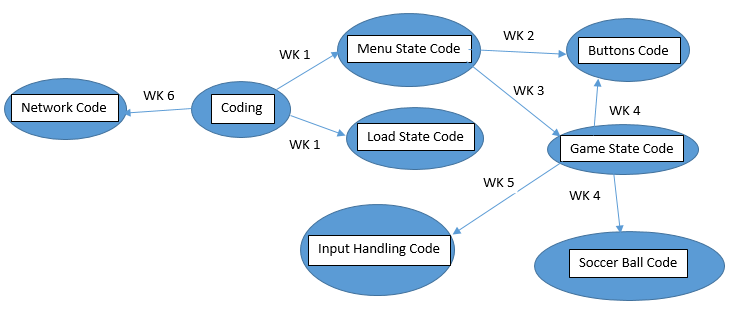
\includegraphics[width=145mm]{Code PERT.png}
\end{center}

\bf{Graphics PERT Chart:}
\begin{center}
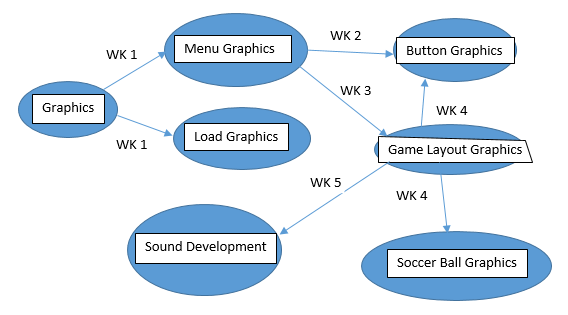
\includegraphics[width=140mm]{Graphics PERT.png}
\end{center}


\subsection{4.4.2 Task / Resource Table}

\begin{center}
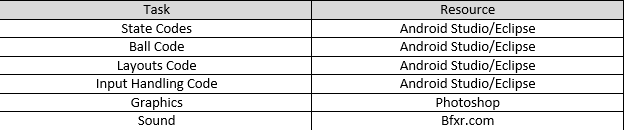
\includegraphics[width=140mm]{Tasks vs Resources.png}
\end{center}

\end{document}